\section{三}

\subsection{三轉四諦}
\begin{itemize}
  \item 示轉:說明此是苦、此是集、此是滅、此是道。
  \item 勸轉:說明苦應知、集應斷、滅應證、道應修。
  \item 證轉:說明苦者我已知、集者我已斷、滅者我已證、道者我已修。
\end{itemize}

\subsection{三苦}
\begin{itemize}
  \item 苦苦
  \item 壞苦
  \item 行苦
\end{itemize}

\subsection{三連鎖}
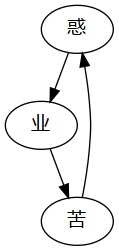
\includegraphics{释家/images/三连锁.png}
\begin{itemize}
  \item 惑:過去世的無明,現在世的愛及取。
  \item 業:過去世的行,現在世的有。
  \item 苦:現在世的識、名色、六入、觸、受,未來世的生及老死。
\end{itemize}
